\documentclass[14pt, aspectratio=169]{beamer}
\usetheme{Copenhagen}
\usecolortheme{beaver}

\setbeamertemplate{navigation symbols}{}

\title{2D Rogue-Like}
\author{Team Cherry}
\date{2022/11/03}

\begin{document}
	\maketitle
	\begin{frame}{Csapattagok}
		\begin{itemize}
			\item Orosz Péter
			\item Dobai Attila
			\item Drahos Alinka
			\item Tőzsér Zétény
			\item Gáncsos Dániel
		\end{itemize}
	\end{frame}

	\begin{frame}{Osztálydiagram}
		\begin{figure}
			\centering
    		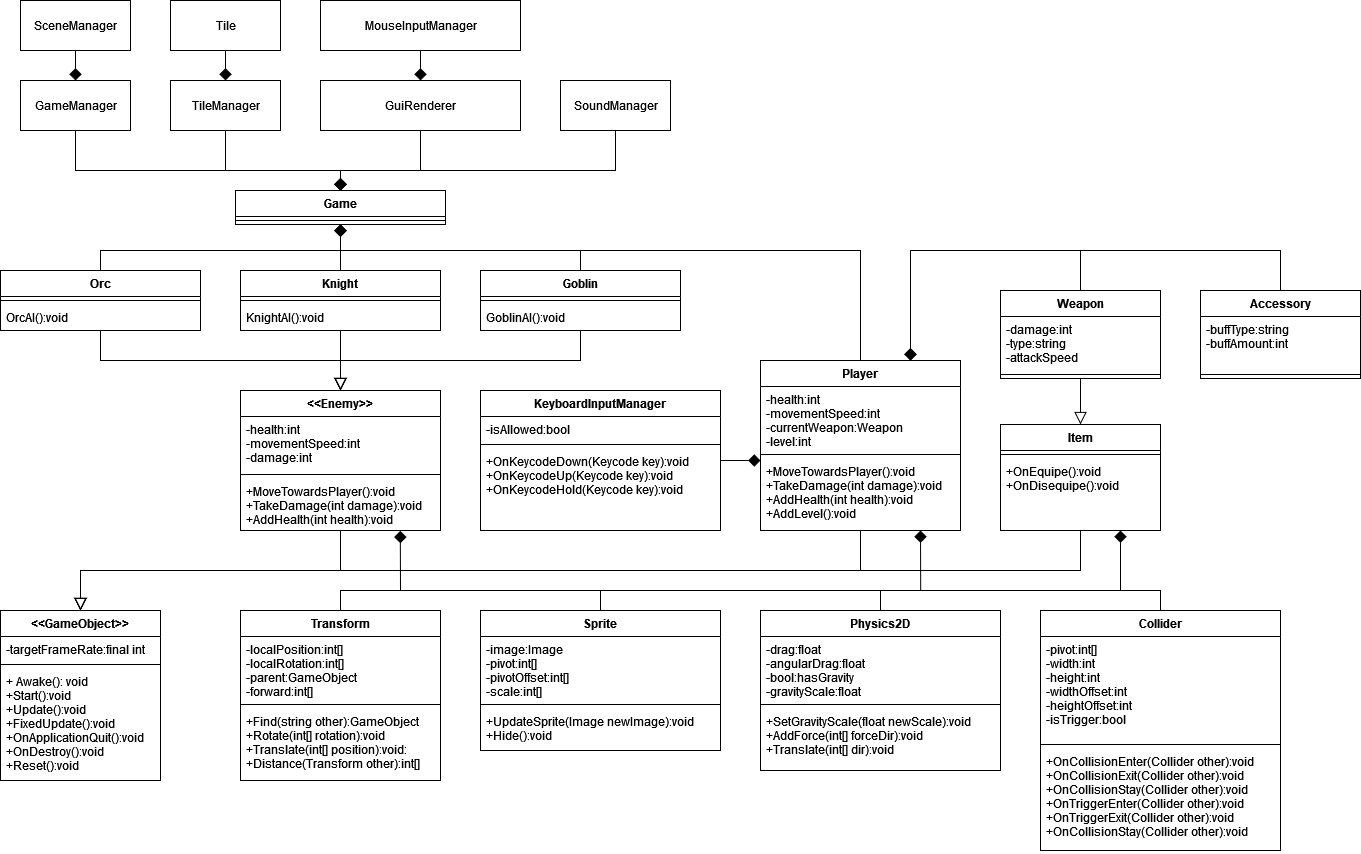
\includegraphics[height = 0.8\textheight]{osztalydiagram.png}
		\end{figure}
	\end{frame}
	
	\begin{frame}{Osztályok}
		\only<1>
		{
			\begin{figure}
				\centering
    			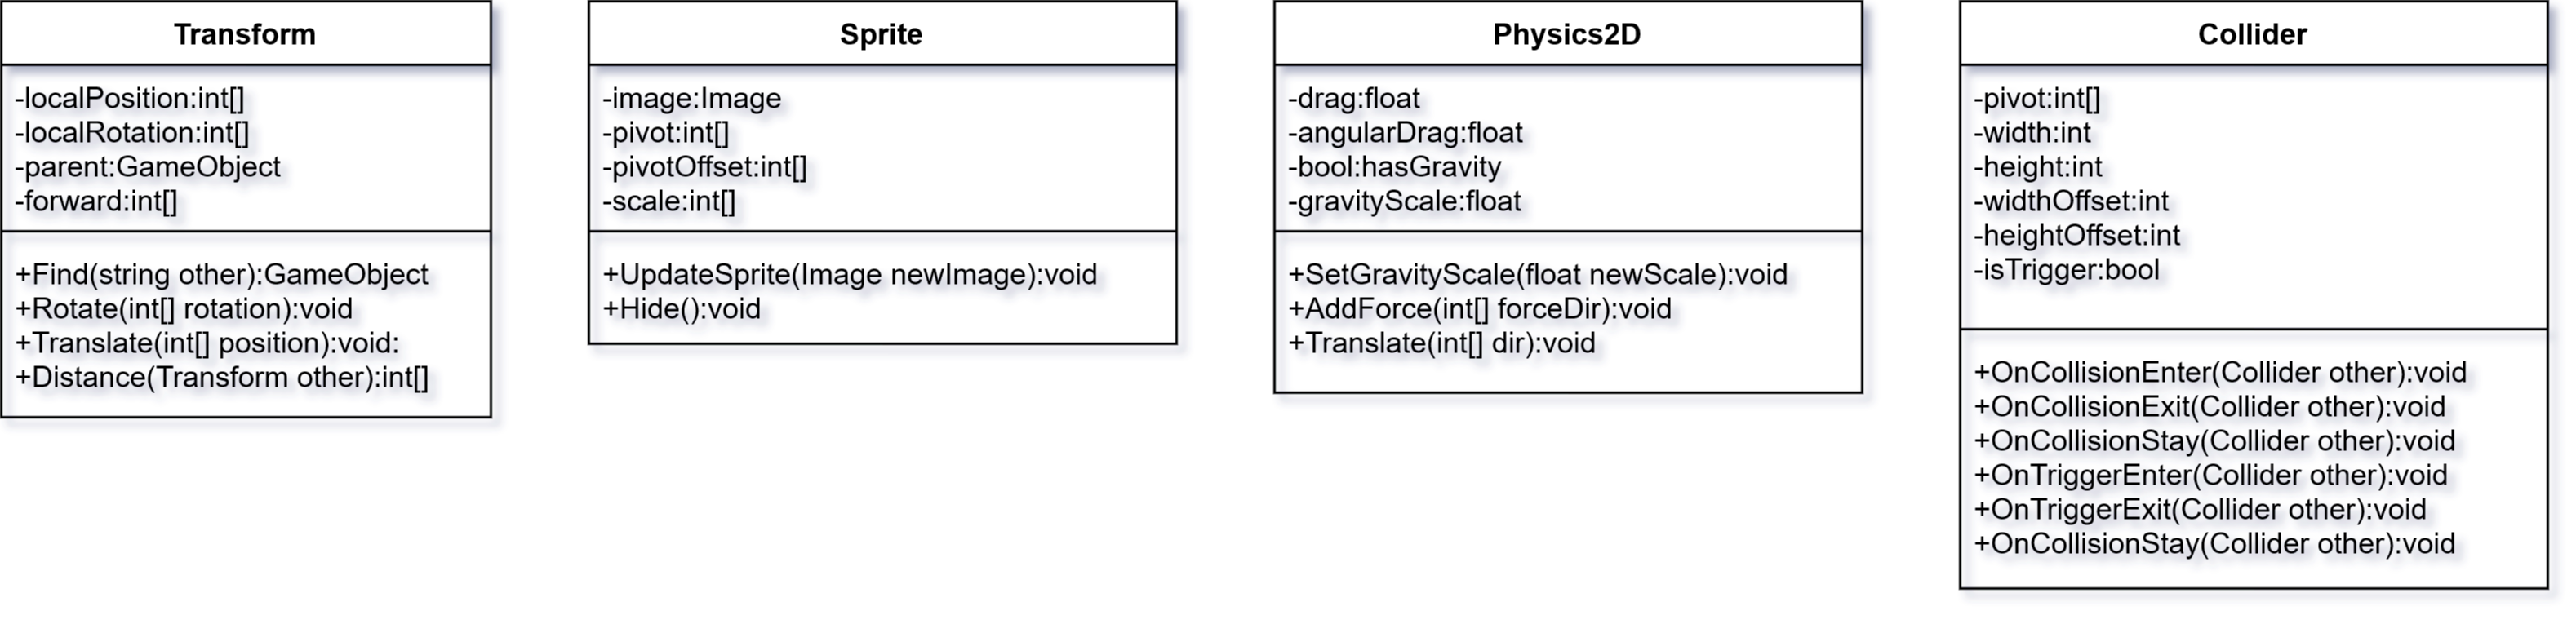
\includegraphics[height = 0.4\textheight]{Tulajdonsagok.png}
			\end{figure}
		}
		\only<2>
		{
			\begin{figure}
				\centering
    			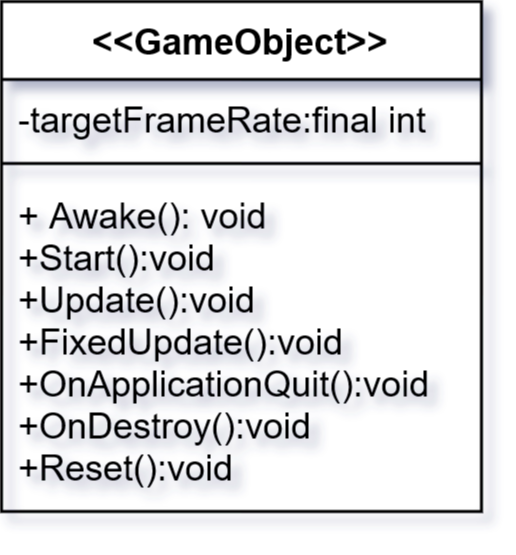
\includegraphics[height = 0.8\textheight]{GameObject.png}
			\end{figure}
		}
		\only<3>
		{
			\begin{figure}
				\centering
    			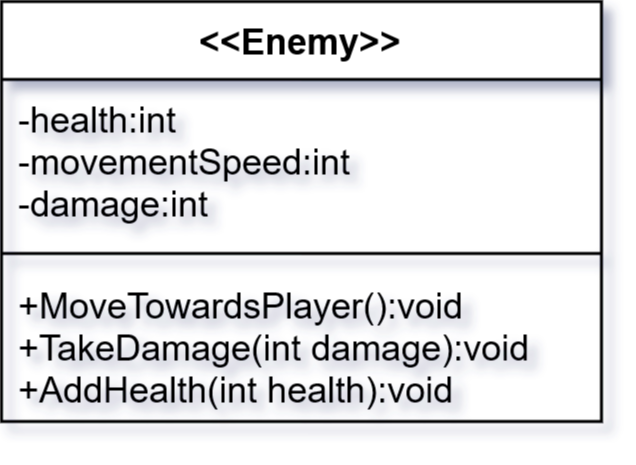
\includegraphics[height = 0.8\textheight]{Enemy.png}
			\end{figure}
		}
		\only<4>
		{
			\begin{figure}
				\centering
    			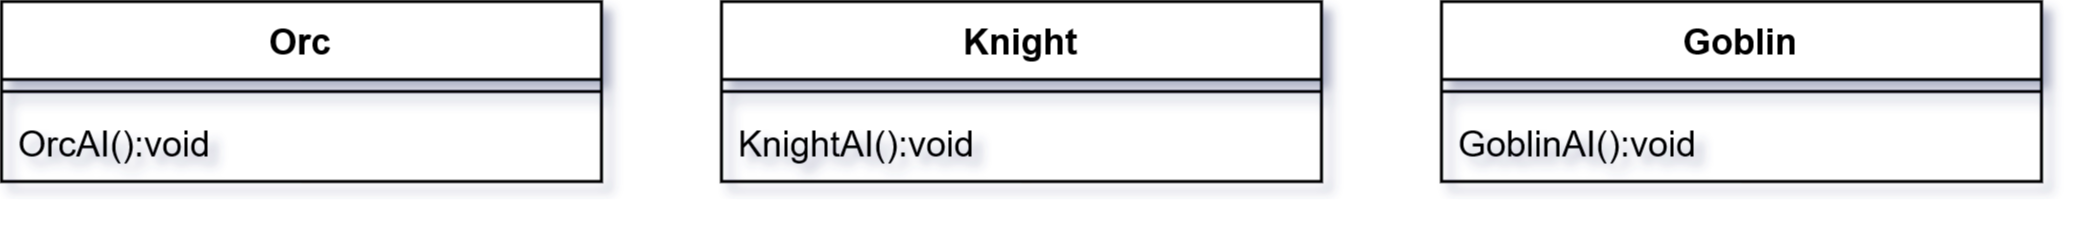
\includegraphics[height = 0.18\textheight]{Enemies.png}
			\end{figure}
		}
		\only<5>
		{
			\begin{figure}
				\centering
    			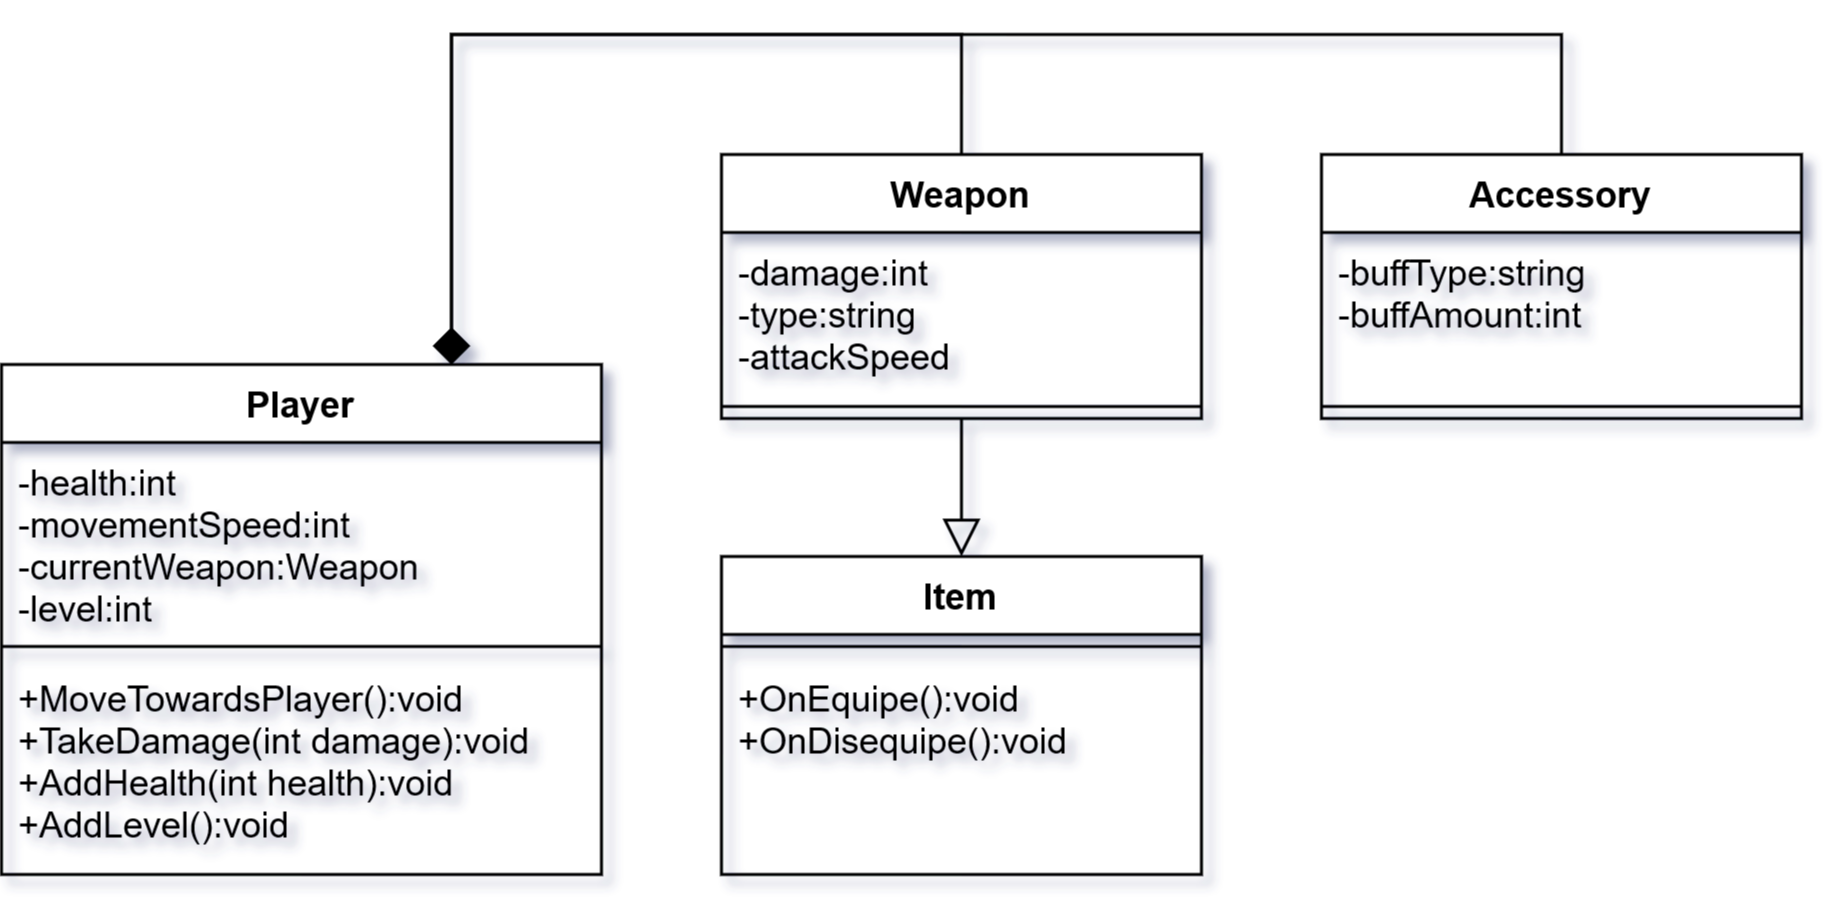
\includegraphics[height = 0.6\textheight]{Player.png}
			\end{figure}
		}
	\end{frame}
\end{document}